\documentclass[11pt,a4paper]{article}

% --- Packages ----------------------------------------------------------------
\usepackage[margin=1.9cm,top=1.8cm,bottom=2.0cm]{geometry}
\usepackage[T1]{fontenc}
\usepackage[utf8]{inputenc}
\usepackage{lmodern}
\usepackage{microtype}
\usepackage{graphicx}
\usepackage{xcolor}
\usepackage{hyperref}
\usepackage{booktabs}
\usepackage{tabularx}
\usepackage{listings}
\usepackage{tikz}
\usepackage{caption}
\usepackage{enumitem}
\usepackage{subcaption}
\usepackage{tcolorbox}

\tcbuselibrary{skins,breakable}

\usetikzlibrary{positioning,shapes.geometric,arrows.meta,calc,fit,backgrounds,chains}

% --- Hyperref colours --------------------------------------------------------
\definecolor{accent}{HTML}{2F4F86}
\definecolor{accent2}{HTML}{C2410C}
\definecolor{accent3}{HTML}{0E7C66}

\hypersetup{
  colorlinks=true,
  linkcolor=accent,
  citecolor=accent,
  urlcolor=accent,
  pdftitle={Enterprise Doc AI: A Local-First Document Question Answering System},
  pdfauthor={Shahab Azmi, Chitransh Kumar Gupta},
}

% --- Listings ----------------------------------------------------------------
\definecolor{codebg}{RGB}{246,248,250}
\definecolor{codecmt}{RGB}{106,115,125}
\definecolor{codekw}{RGB}{215,58,73}
\definecolor{codestr}{RGB}{32,113,69}

\lstdefinestyle{py}{
  backgroundcolor=\color{codebg},
  basicstyle=\ttfamily\footnotesize,
  commentstyle=\color{codecmt}\itshape,
  keywordstyle=\color{codekw}\bfseries,
  stringstyle=\color{codestr},
  language=Python,
  numbers=none,
  breaklines=true,
  frame=single,
  framesep=4pt,
  rulecolor=\color{black!18},
  showstringspaces=false,
  tabsize=2,
  aboveskip=5pt,
  belowskip=5pt,
}

% --- Caption styling ---------------------------------------------------------
\captionsetup{font=small,labelfont=bf,format=plain,labelsep=period}
\setlength{\parskip}{2pt}
\setlength{\textfloatsep}{6pt plus 1pt minus 1pt}
\setlength{\intextsep}{6pt plus 1pt minus 1pt}
\setlength{\abovecaptionskip}{4pt}

% --- Problem/fix box ---------------------------------------------------------
\newtcolorbox{problembox}[1]{%
  enhanced, breakable, sharp corners,
  colback=accent2!5, colframe=accent2!70, boxrule=0.4pt,
  left=6pt, right=6pt, top=4pt, bottom=4pt,
  fonttitle=\bfseries\small\color{white},
  coltitle=white,
  colbacktitle=accent2!85,
  attach boxed title to top left={xshift=4pt,yshift=-2pt},
  boxed title style={sharp corners,boxrule=0pt},
  title={#1},
}

% --- Title -------------------------------------------------------------------
\title{
  \vspace{-1.0cm}
  \textbf{Enterprise Doc AI}\\
  \vspace{2pt}
  \large A Local-First Document Question Answering System\\
  \normalsize\emph{Project summary, lessons learned, and a live demo on three real PDFs}
}
\author{Shahab Azmi \quad\textperiodcentered\quad Chitransh Kumar Gupta}
\date{May 2026}

\begin{document}
\maketitle
\vspace{-0.7cm}

% =============================================================================
\begin{abstract}
\noindent
Public AI assistants like ChatGPT cannot be trusted with private files such as
contracts, financial reports, or government documents because the file must
be uploaded to a third-party server. \textbf{Enterprise Doc AI} solves this by
running the \emph{entire} question-answering pipeline on a single laptop. A
user uploads a PDF (or DOCX, TXT, image) through a Streamlit chat interface,
asks a question in English, and gets a grounded answer with source citations
-- all on an Apple~M2 with 8\,GB of RAM, no GPU, and no internet at query
time. This report is the story of how the system was built. It walks through
the architecture, the upload pipeline, the query pipeline, the specific
\emph{retrieval, hallucination, and grounding} problems hit along the way and
how each was fixed in code, and a live evaluation on the NVIDIA~2025 Annual
Report (1{,}631 chunks), the Tesla Form~10-K~2024 (1{,}180 chunks), and the
FBI~NCIC Privacy Impact Assessment (259 chunks) -- 3{,}070 chunks indexed in
a single Milvus~Lite file.
\end{abstract}

% =============================================================================
\section{Introduction and Motivation}
\label{sec:intro}

Large language models such as GPT-4 or Claude can read a document and answer
questions about it, but they have three real-world problems for everyday
users.

\begin{itemize}[leftmargin=18pt,topsep=2pt,itemsep=2pt]
  \item \textbf{Privacy.} Hosted LLMs require the user to upload the
        document. That is unacceptable for confidential material -- legal
        contracts, medical records, or government privacy assessments like
        the FBI NCIC PIA we used in our evaluation.
  \item \textbf{Hallucination.} A plain LLM, asked about a fact it has not
        seen, will confidently make one up. Even hosted retrieval-augmented
        services rarely show \emph{which sentence} grounded the answer.
  \item \textbf{Cost.} Paid APIs charge per page indexed and per question
        asked, which is wasteful for a student running a few documents on a
        laptop.
\end{itemize}

\noindent
Our goal was to build a complete document question-answering system that
fixes all three issues at once by being \emph{local-first}: the parser, the
keyword index, the embeddings, the LLM, and the conversation history all
live on the user's machine. The system was developed and tested on an Apple
M2 laptop with 8\,GB of RAM and no discrete GPU. Once the model files are
pulled, the laptop can be disconnected from the internet and the system
still works end-to-end.

\paragraph{What the system does, in one paragraph.}
The user opens a Streamlit chat page, uploads one or more files, and asks a
question. The backend decides whether the question is about an uploaded
document, ordinary chat, or a live-data request (``what's the weather in
Moscow?''). If the question is about a document, the backend retrieves the
three to seven most relevant chunks using a combination of keyword and
semantic search, builds a strict grounded prompt, calls the local LLM, and
returns the answer along with the source pages so the user can verify it.

% =============================================================================
\section{System Architecture}
\label{sec:arch}

\begin{figure}[h]
\centering
\resizebox{0.96\linewidth}{!}{%
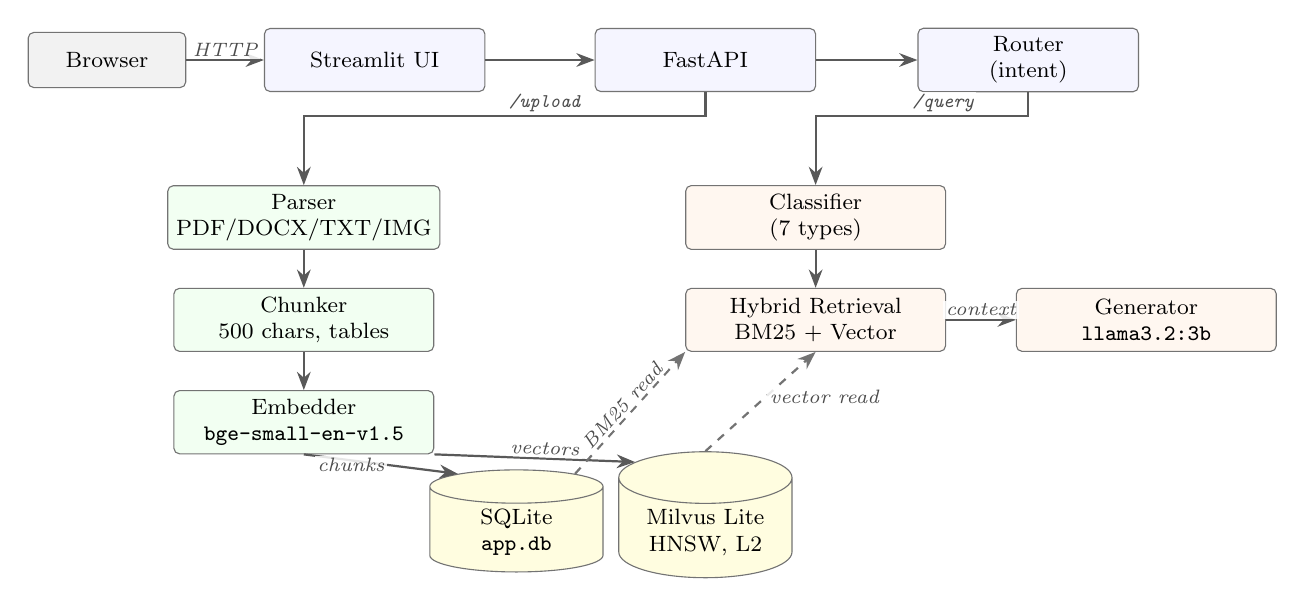
\begin{tikzpicture}[
  every node/.style={font=\footnotesize,align=center},
  block/.style={rectangle,draw=black!55,rounded corners=2pt,minimum width=28mm,
                minimum height=8mm,inner sep=3pt,fill=blue!4},
  ingblk/.style={rectangle,draw=black!55,rounded corners=2pt,minimum width=33mm,
                 minimum height=8mm,inner sep=3pt,fill=green!5},
  qryblk/.style={rectangle,draw=black!55,rounded corners=2pt,minimum width=33mm,
                 minimum height=8mm,inner sep=3pt,fill=orange!6},
  store/.style={cylinder,shape border rotate=90,draw=black!55,minimum width=22mm,
                minimum height=10mm,inner sep=2pt,aspect=0.4,fill=yellow!12},
  user/.style ={rectangle,rounded corners=2pt,draw=black!55,minimum width=20mm,
                minimum height=7mm,fill=gray!10},
  arr/.style  ={-Stealth,thick,black!65},
  rdarr/.style={-Stealth,thick,black!55,dashed},
  lab/.style  ={font=\scriptsize\itshape,black!70,inner sep=1pt,fill=white,
                fill opacity=0.85,text opacity=1},
]
\node[user]   at (0,    0)    (browser)   {Browser};
\node[block]  at (3.4,  0)    (st)        {Streamlit UI};
\node[block]  at (7.6,  0)    (api)       {FastAPI};
\node[block]  at (11.7, 0)    (router)    {Router\\(intent)};

\node[ingblk] at (2.5, -2.0)  (parse)     {Parser\\PDF/DOCX/TXT/IMG};
\node[ingblk] at (2.5, -3.3)  (chunk)     {Chunker\\500 chars, tables};
\node[ingblk] at (2.5, -4.6)  (embed)     {Embedder\\\texttt{bge-small-en-v1.5}};

\node[qryblk] at (9.0, -2.0)  (classify)  {Classifier\\(7 types)};
\node[qryblk] at (9.0, -3.3)  (retrieve)  {Hybrid Retrieval\\BM25 + Vector};
\node[qryblk] at (13.2,-3.3)  (gen)       {Generator\\\texttt{llama3.2:3b}};

\node[store]  at (5.2, -6.0)  (sqlite)    {SQLite\\\texttt{app.db}};
\node[store]  at (7.6, -6.0)  (milvus)    {Milvus Lite\\HNSW, L2};

\draw[arr] (browser.east) -- node[lab,above]{HTTP} (st.west);
\draw[arr] (st.east)      -- (api.west);
\draw[arr] (api.east)     -- (router.west);

\draw[arr] (api.south) -- ++(0,-3mm) -|
  node[lab,pos=0.2,above]{\texttt{/upload}} (parse.north);
\draw[arr] (router.south) -- ++(0,-3mm) -|
  node[lab,pos=0.2,above]{\texttt{/query}}  (classify.north);

\draw[arr] (parse) -- (chunk);
\draw[arr] (chunk) -- (embed);
\draw[arr] (classify) -- (retrieve);
\draw[arr] (retrieve.east) -- node[lab,above]{context} (gen.west);

\draw[arr] (embed.south)
  -- node[lab,left,pos=0.55]{chunks} (sqlite.north west);
\draw[arr] (embed.south east)
  -- node[lab,above,sloped,pos=0.55]{vectors} (milvus.north west);

\draw[rdarr] (sqlite.north east)
  -- node[lab,above,sloped,pos=0.5]{BM25 read} (retrieve.south west);
\draw[rdarr] (milvus.north)
  -- node[lab,right,pos=0.55]{vector read} (retrieve.south);
\end{tikzpicture}%
}
\caption{End-to-end architecture. The \textcolor{green!50!black}{green} column
is the \emph{upload} path: parse, chunk, embed, then write text to SQLite and
vectors to Milvus. The \textcolor{orange!70!black}{orange} column is the
\emph{query} path: classify, fuse keyword and vector hits, build context,
call the LLM. SQLite is the single source of truth; the vector store is
rebuilt from it on startup if the file is missing.}
\label{fig:arch}
\end{figure}

\paragraph{Three design principles.}
(i)~The system must work fully \emph{offline} once the models are pulled.
(ii)~Document content must \emph{never} leave the device.
(iii)~All state -- documents, chunks, and conversation history -- must
\emph{survive a server restart} without manual repair.

% =============================================================================
\section{Step 1: The Upload Pipeline}
\label{sec:upload}

When the user drops a file into the chat box, \texttt{POST /upload} runs
five steps. Figure~\ref{fig:upload-journey} traces the journey for the Tesla
Form~10-K (a 1.7\,MB PDF we tested).

\begin{figure}[h]
\centering
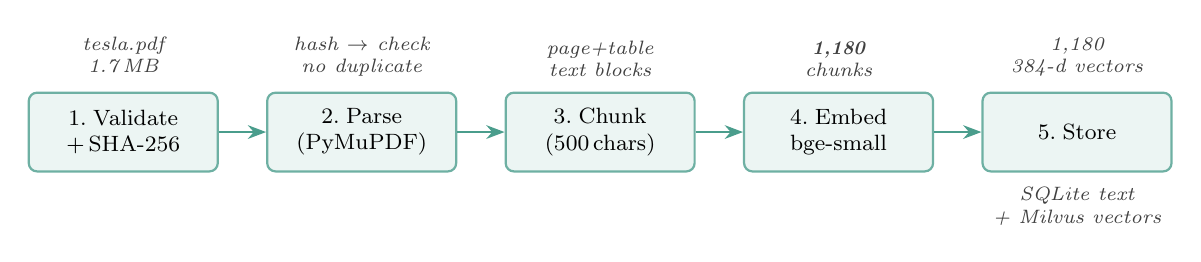
\begin{tikzpicture}[
  every node/.style={font=\footnotesize,align=center},
  ustep/.style={rectangle,draw=accent3!60,rounded corners=3pt,
               minimum width=24mm,minimum height=10mm,inner sep=4pt,
               fill=accent3!8,thick},
  data/.style={font=\scriptsize\itshape,align=center,text=black!75},
  arr/.style ={-Stealth,thick,accent3!75},
]
\node[ustep] (s1) {1.\;Validate\\+\,SHA-256};
\node[ustep,right=6mm of s1] (s2) {2.\;Parse\\(PyMuPDF)};
\node[ustep,right=6mm of s2] (s3) {3.\;Chunk\\(500\,chars)};
\node[ustep,right=6mm of s3] (s4) {4.\;Embed\\bge-small};
\node[ustep,right=6mm of s4] (s5) {5.\;Store};

\node[data,above=2pt of s1] {tesla.pdf\\1.7\,MB};
\node[data,above=2pt of s2] {hash $\to$ check\\no duplicate};
\node[data,above=2pt of s3] {page+table\\text blocks};
\node[data,above=2pt of s4] {\textbf{1{,}180}\\chunks};
\node[data,above=2pt of s5] {1{,}180\\384-d vectors};
\node[data,below=2pt of s5] {SQLite text\\+ Milvus vectors};

\draw[arr] (s1) -- (s2);
\draw[arr] (s2) -- (s3);
\draw[arr] (s3) -- (s4);
\draw[arr] (s4) -- (s5);
\end{tikzpicture}
\caption{The journey of \texttt{NASDAQ\_TSLA\_2024.pdf} through the upload
pipeline. The italic labels above and below each step show what the data
actually looks like at that point. Total wall-clock time:
$\approx\!40$\,s on an Apple~M2.}
\label{fig:upload-journey}
\end{figure}

\noindent
The steps are: \textbf{(1)}~validate the extension and SHA-256-hash the
bytes (an identical file is reused without re-ingesting);
\textbf{(2)}~parse with PyMuPDF page-by-page, extracting tables as separate
elements; \textbf{(3)}~group by page and split with LangChain's
\texttt{RecursiveCharacterTextSplitter} (500 chars, 100 overlap), inheriting
metadata; \textbf{(4)}~embed every chunk with \texttt{BAAI/bge-small-en-v1.5}
(33\,M params, 384-d output); \textbf{(5)}~write the chunks to SQLite and
the vectors to Milvus~Lite in one atomic call.

% =============================================================================
\section{Step 2: The Query Pipeline}
\label{sec:query}

A single \texttt{POST /query} runs four stages. Figure~\ref{fig:query-journey}
traces the real test question \textit{``Who is the CEO of NVIDIA?''} through
the live system.

\begin{figure}[h]
\centering
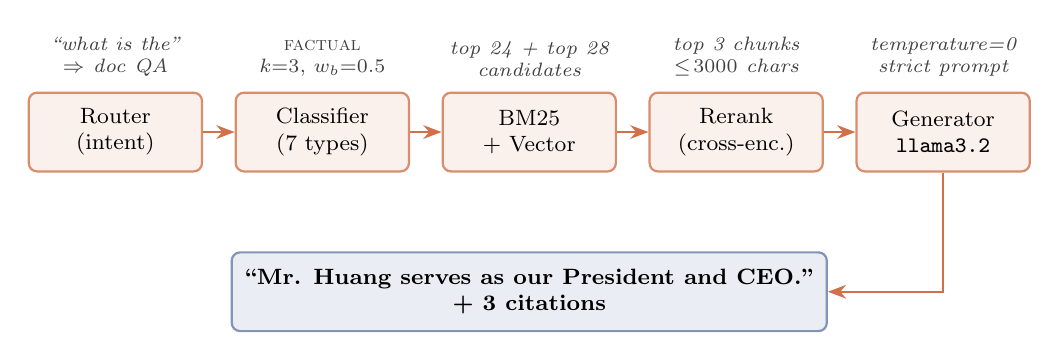
\begin{tikzpicture}[
  every node/.style={font=\footnotesize,align=center},
  qstep/.style={rectangle,draw=accent2!60,rounded corners=3pt,
               minimum width=22mm,minimum height=10mm,inner sep=4pt,
               fill=accent2!8,thick},
  outbox/.style={rectangle,draw=accent!60,rounded corners=3pt,
               minimum width=30mm,minimum height=10mm,inner sep=4pt,
               fill=accent!10,thick,font=\footnotesize\bfseries},
  data/.style={font=\scriptsize\itshape,align=center,text=black!75},
  arr/.style ={-Stealth,thick,accent2!75},
]
\node[qstep] (q1) {Router\\(intent)};
\node[qstep,right=4mm of q1] (q2) {Classifier\\(7 types)};
\node[qstep,right=4mm of q2] (q3) {BM25\\+ Vector};
\node[qstep,right=4mm of q3] (q4) {Rerank\\(cross-enc.)};
\node[qstep,right=4mm of q4] (q5) {Generator\\\texttt{llama3.2}};
\node[outbox,below=10mm of q3] (out) {``Mr. Huang serves as our President and CEO.''\\+ 3 citations};

\node[data,above=2pt of q1] {``what is the''\\$\Rightarrow$ doc QA};
\node[data,above=2pt of q2] {\textsc{factual}\\$k{=}3,\,w_b{=}0.5$};
\node[data,above=2pt of q3] {top 24 + top 28\\candidates};
\node[data,above=2pt of q4] {top 3 chunks\\$\leq\!3000$ chars};
\node[data,above=2pt of q5] {temperature=0\\strict prompt};

\draw[arr] (q1) -- (q2);
\draw[arr] (q2) -- (q3);
\draw[arr] (q3) -- (q4);
\draw[arr] (q4) -- (q5);
\draw[arr] (q5.south) |- (out.east);
\end{tikzpicture}
\caption{The journey of the question \textit{``Who is the CEO of NVIDIA?''}.
The router sees the ``what is the$\dots$'' starter and routes to document
QA; the classifier tags the query as \textsc{factual} with $k{=}3$ and BM25
weight $0.5$; BM25 surfaces the chunk containing the literal phrase
``Mr. Huang \ldots President and CEO'' from page~30 of the NVIDIA report; a
cross-encoder reranks the three best candidates; the generator builds a
strict prompt from those three chunks and emits the four-word
answer.}
\label{fig:query-journey}
\end{figure}

\paragraph{Why classification matters.}
The seven query types (\textsc{extractive}, \textsc{provenance},
\textsc{numerical}, \textsc{list}, \textsc{reasoning}, \textsc{summary},
\textsc{factual}) each tune three knobs: $k$ (how many chunks to retrieve),
$w_b$ (BM25 weight vs.\ vector weight), and $n_\textrm{predict}$ (LLM token
budget). Two of the seven -- \textsc{extractive} and \textsc{provenance} --
skip the LLM call entirely. An extractive query returns the top chunk
verbatim; a provenance query returns only the source/page/section line.
That single decision shaves 5--10 seconds off such queries and removes the
risk of the small model paraphrasing a quote --- a concrete design choice
we made after seeing the 3\,B model paraphrase a verbatim NCIC paragraph
during testing.

\paragraph{Hybrid retrieval, in plain language.}
Stage three of the query pipeline runs \emph{two searches in parallel} ---
keyword search (BM25) finds chunks that contain the literal words of the
question; semantic search (Milvus, over the 384-dim BGE vectors) finds
chunks whose meaning matches the question. Their candidate lists are
unioned and scored together. We tried each search alone first --- both
missed obvious answers when used in isolation --- which is why the
production system uses the fused score:
$\mathrm{score}(d) = w_b\,\widehat{b}(d) + (1-w_b)\,\widehat{r}(d) + \beta(q,d)$,
where $\widehat{b}$ is the min--max-normalised BM25 score, $\widehat{r}$
is the normalised inverse vector rank, and $\beta$ adds small domain
bonuses (a page-1 boost for instructor / CEO questions, an
\texttt{@}-token bonus for contact queries, a parenthetical-acronym match
for short keywords like ``NLP'' inside ``Natural Language Processing
(NLP)''). A cross-encoder then re-scores the top candidates by reading
each chunk \emph{together with} the question --- slower than the two
initial searches, but much sharper.

% =============================================================================
\section{What Broke When We Tested, and How We Fixed It}
\label{sec:problems}

The first version of every component was naive and broke in obvious ways
the moment we ran a real PDF through it. The interesting engineering
happened in the second and third iterations. Each problem below is tied to
a specific test we ran against one of the three corpus PDFs (NVIDIA
Annual Report, Tesla 10-K, FBI NCIC Privacy Impact Assessment) and
followed the same shape: \emph{Test} (what we asked) $\to$ \emph{Bug}
(what the system did wrong) $\to$ \emph{Diagnosis} (why it broke)
$\to$ \emph{Fix} (the change in code) $\to$ \emph{After} (what the system
returns now).

\begin{problembox}{Problem 1 -- Tesla 10-K: revenue queries returned nonsense (\,table collapse)}
\textbf{Test.}
\textit{``What was Tesla's total automotive revenue in 2024?''}\\[2pt]
\textbf{Bug.}
The first version returned a confused string of digits taken from the
wrong column. The right number existed in the PDF but the LLM could not
pick out which year.\\[2pt]
\textbf{Diagnosis.}
PyMuPDF read the table cells correctly, but our chunker's
\texttt{\_normalize\_chunk\_text} helper collapsed \emph{all} whitespace
into single spaces. A row like
\texttt{Automotive\;21,344\;23,210\;17,933\;25,500} that spans four year
columns became one indistinguishable line of digits -- BM25 tokens looked
like gibberish and the embedder saw a wall of numbers.\\[2pt]
\textbf{Fix (\texttt{backend/services/chunker.py}).}
A 6-line heuristic detects ``table-like'' blocks: if a chunk has at least
three lines and more than~40\,\% of them are short ($<\!80$ chars) and
contain a digit, preserve the line breaks instead of collapsing them.\\[2pt]
\textbf{After.}
The same question now returns \textbf{``\$77{,}070 million.''} with three
source citations pointing back to the Tesla revenue tables.
\end{problembox}

\begin{problembox}{Problem 2 -- NVIDIA Annual Report: hallucinated hedge phrases}
\textbf{Test.}
\textit{``Who is the CEO of NVIDIA?''}\\[2pt]
\textbf{Bug.}
The 3\,B LLM \emph{did} pick up the right chunk, but its first version of
the answer looked like this:
\textit{``Based on the provided document, NVIDIA's leadership could lead
to further growth\ldots analysts believe Mr.~Huang\ldots''} -- two hedge
phrases that do not appear anywhere in the document.\\[2pt]
\textbf{Diagnosis.}
A small instruction-tuned model is trained to sound helpful, and
``helpful'' includes confident-sounding openers and hedge phrases. A
grounded context alone does not suppress those habits.\\[2pt]
\textbf{Fix (\texttt{backend/services/generator.py}).}
Three layers of defence:
\textbf{(a)} a 10-rule system prompt that bans outside knowledge and
forces the reply \textit{``I could not find this information in the
document''} when the context is silent;
\textbf{(b)} per-type addenda -- the \textsc{reasoning} addendum
explicitly forbids the phrases ``could lead to'', ``analysts believe'',
and ``market trends suggest'';
\textbf{(c)} a regex post-processor (\texttt{\_GENERIC\_OPENERS\_RE}) that
strips ``Based on the document\ldots'' and similar openers from the model
output before returning it.\\[2pt]
\textbf{After.}
\textit{``Mr.\ Huang serves as our President and CEO.''} -- exactly seven
words, taken from the chunk on page~30 of the NVIDIA Annual Report.
\end{problembox}

\begin{problembox}{Problem 3 -- NCIC PIA: verbatim paragraphs got paraphrased}
\textbf{Test.}
\textit{``Show me the exact paragraph about the NCIC system administrator
role.''}\\[2pt]
\textbf{Bug.}
Even with strict prompts the 3\,B model re-worded the paragraph instead of
quoting it word-for-word.\\[2pt]
\textbf{Diagnosis.}
An instruction-tuned generative model defaults to summarising. Once the
model has the paragraph in its context, prompts alone don't fully prevent
paraphrasing.\\[2pt]
\textbf{Fix (\texttt{backend/services/query\_classifier.py},
\texttt{generator.py}).}
The \textsc{extractive} and \textsc{provenance} query types bypass the LLM
\emph{entirely}. An extractive query returns the top retrieved chunk
verbatim, with a citation; a provenance query returns only the
file/page/section metadata.\\[2pt]
\textbf{After.}
The exact paragraph is returned in $\approx\!200$\,ms (instead of
5--10\,s with the LLM in the loop) and is 100\,\% faithful to the
PDF.
\end{problembox}

\begin{problembox}{Problem 4 -- Retrieval: the bi-encoder kept missing the obvious chunk}
\textbf{Test.}
\textit{``Who is the instructor of the NLP course?''} (and, by analogy,
\textit{``Who is the CEO of NVIDIA?''}).\\[2pt]
\textbf{Bug.}
A pure semantic search returned vaguely-related chunks but missed the page
that started with the literal word \texttt{Instructor:} (or
\texttt{President\,\&\,CEO:}).\\[2pt]
\textbf{Diagnosis.}
Small bi-encoders like \texttt{bge-small} encode meaning, not exact
wording. A page-1 chunk that begins with \texttt{Instructor: Assoc.\ Prof.
Soroosh Shalileh} is the right answer but does not have higher cosine
similarity than mid-document course-policy paragraphs.\\[2pt]
\textbf{Fix (\texttt{backend/services/retrieval.py}).}
We added \emph{hybrid retrieval}: BM25 keyword search runs in parallel
with vector search, the two pools are fused with a weighted convex
combination, and a cross-encoder picks the sharpest match. Small
domain-aware bonuses give +0.10 to page-1 chunks for instructor / CEO
queries, +0.12 to chunks containing \texttt{@}, and +0.18 for
parenthetical-acronym matches like ``NLP'' inside
``Natural Language Processing~(NLP)''.\\[2pt]
\textbf{After.}
The instructor / CEO chunk ranks first on BM25 alone, and the
cross-encoder confirms it -- visible in the NVIDIA screenshot in the
next section.
\end{problembox}

\paragraph{Problem 5 -- State loss and long-context decay (two smaller wins).}
\textbf{Context overflow.} Filling the model's full $\approx\!4$\,k token
context with retrieved chunks actually \emph{hurt} answer quality -- the
3\,B model would forget the question buried under the retrieved noise. We
capped retrieved context at 3{,}000 characters and quality improved
measurably.
\textbf{State loss.} On a Mac sleep/wake cycle Milvus Lite would sometimes
drop its connection (\textit{``should create connection first''}). We
catch that specific error string, reset the store, and retry the call;
separately, we rebuild the vector store from SQLite on every startup if
the Milvus file is missing, so the user can delete
\texttt{milvus\_demo.db} and the next \texttt{/query} still works.

% =============================================================================
\section{Live Evaluation on Three Real PDFs}
\label{sec:eval}

\paragraph{Why these three PDFs.}
We deliberately picked PDFs that stress \emph{different parts} of the
pipeline: the \textbf{NVIDIA 2025 Annual Report} (tech industry, dense
prose, long document at 1{,}631~chunks) tests retrieval scale and the
hallucination guard; the \textbf{Tesla Form 10-K (FY 2024)} (1{,}180
chunks, financial-table heavy) tests the table-aware chunker; the
\textbf{FBI NCIC Privacy Impact Assessment} (259 chunks, US government
document with formal language) tests reasoning over open-ended
``what is the purpose of $X$'' questions. All three are indexed at once
in a single Milvus Lite file (3{,}070 chunks total) and the system
chooses the right corpus material per query via hybrid retrieval, with no
manual document selection.

Figure~\ref{fig:demos} shows three real answers, one from each PDF, and
Figure~\ref{fig:multiturn} shows a single conversation that crosses two
routing branches.

\begin{table}[h]
\centering
\small
\caption{Indexed corpus during the live evaluation. Chunk counts are
reported by \texttt{GET /documents}.}
\label{tab:corpus}
\begin{tabularx}{0.85\linewidth}{@{}Xllr@{}}
\toprule
Document & Domain & Format & Chunks \\
\midrule
NVIDIA Corporation 2025 Annual Report     & Tech / SEC filing  & PDF  & 1{,}631 \\
Tesla, Inc.\ Form 10-K (FY 2024)          & Auto / SEC filing  & PDF  & 1{,}180 \\
FBI NCIC Privacy Impact Assessment        & US government PIA  & PDF  & 259 \\
\midrule
\textbf{Total}                            &                    &      & \textbf{3{,}070} \\
\bottomrule
\end{tabularx}
\end{table}

\begin{figure}[h]
\centering
\begin{subcaptionblock}{0.32\textwidth}
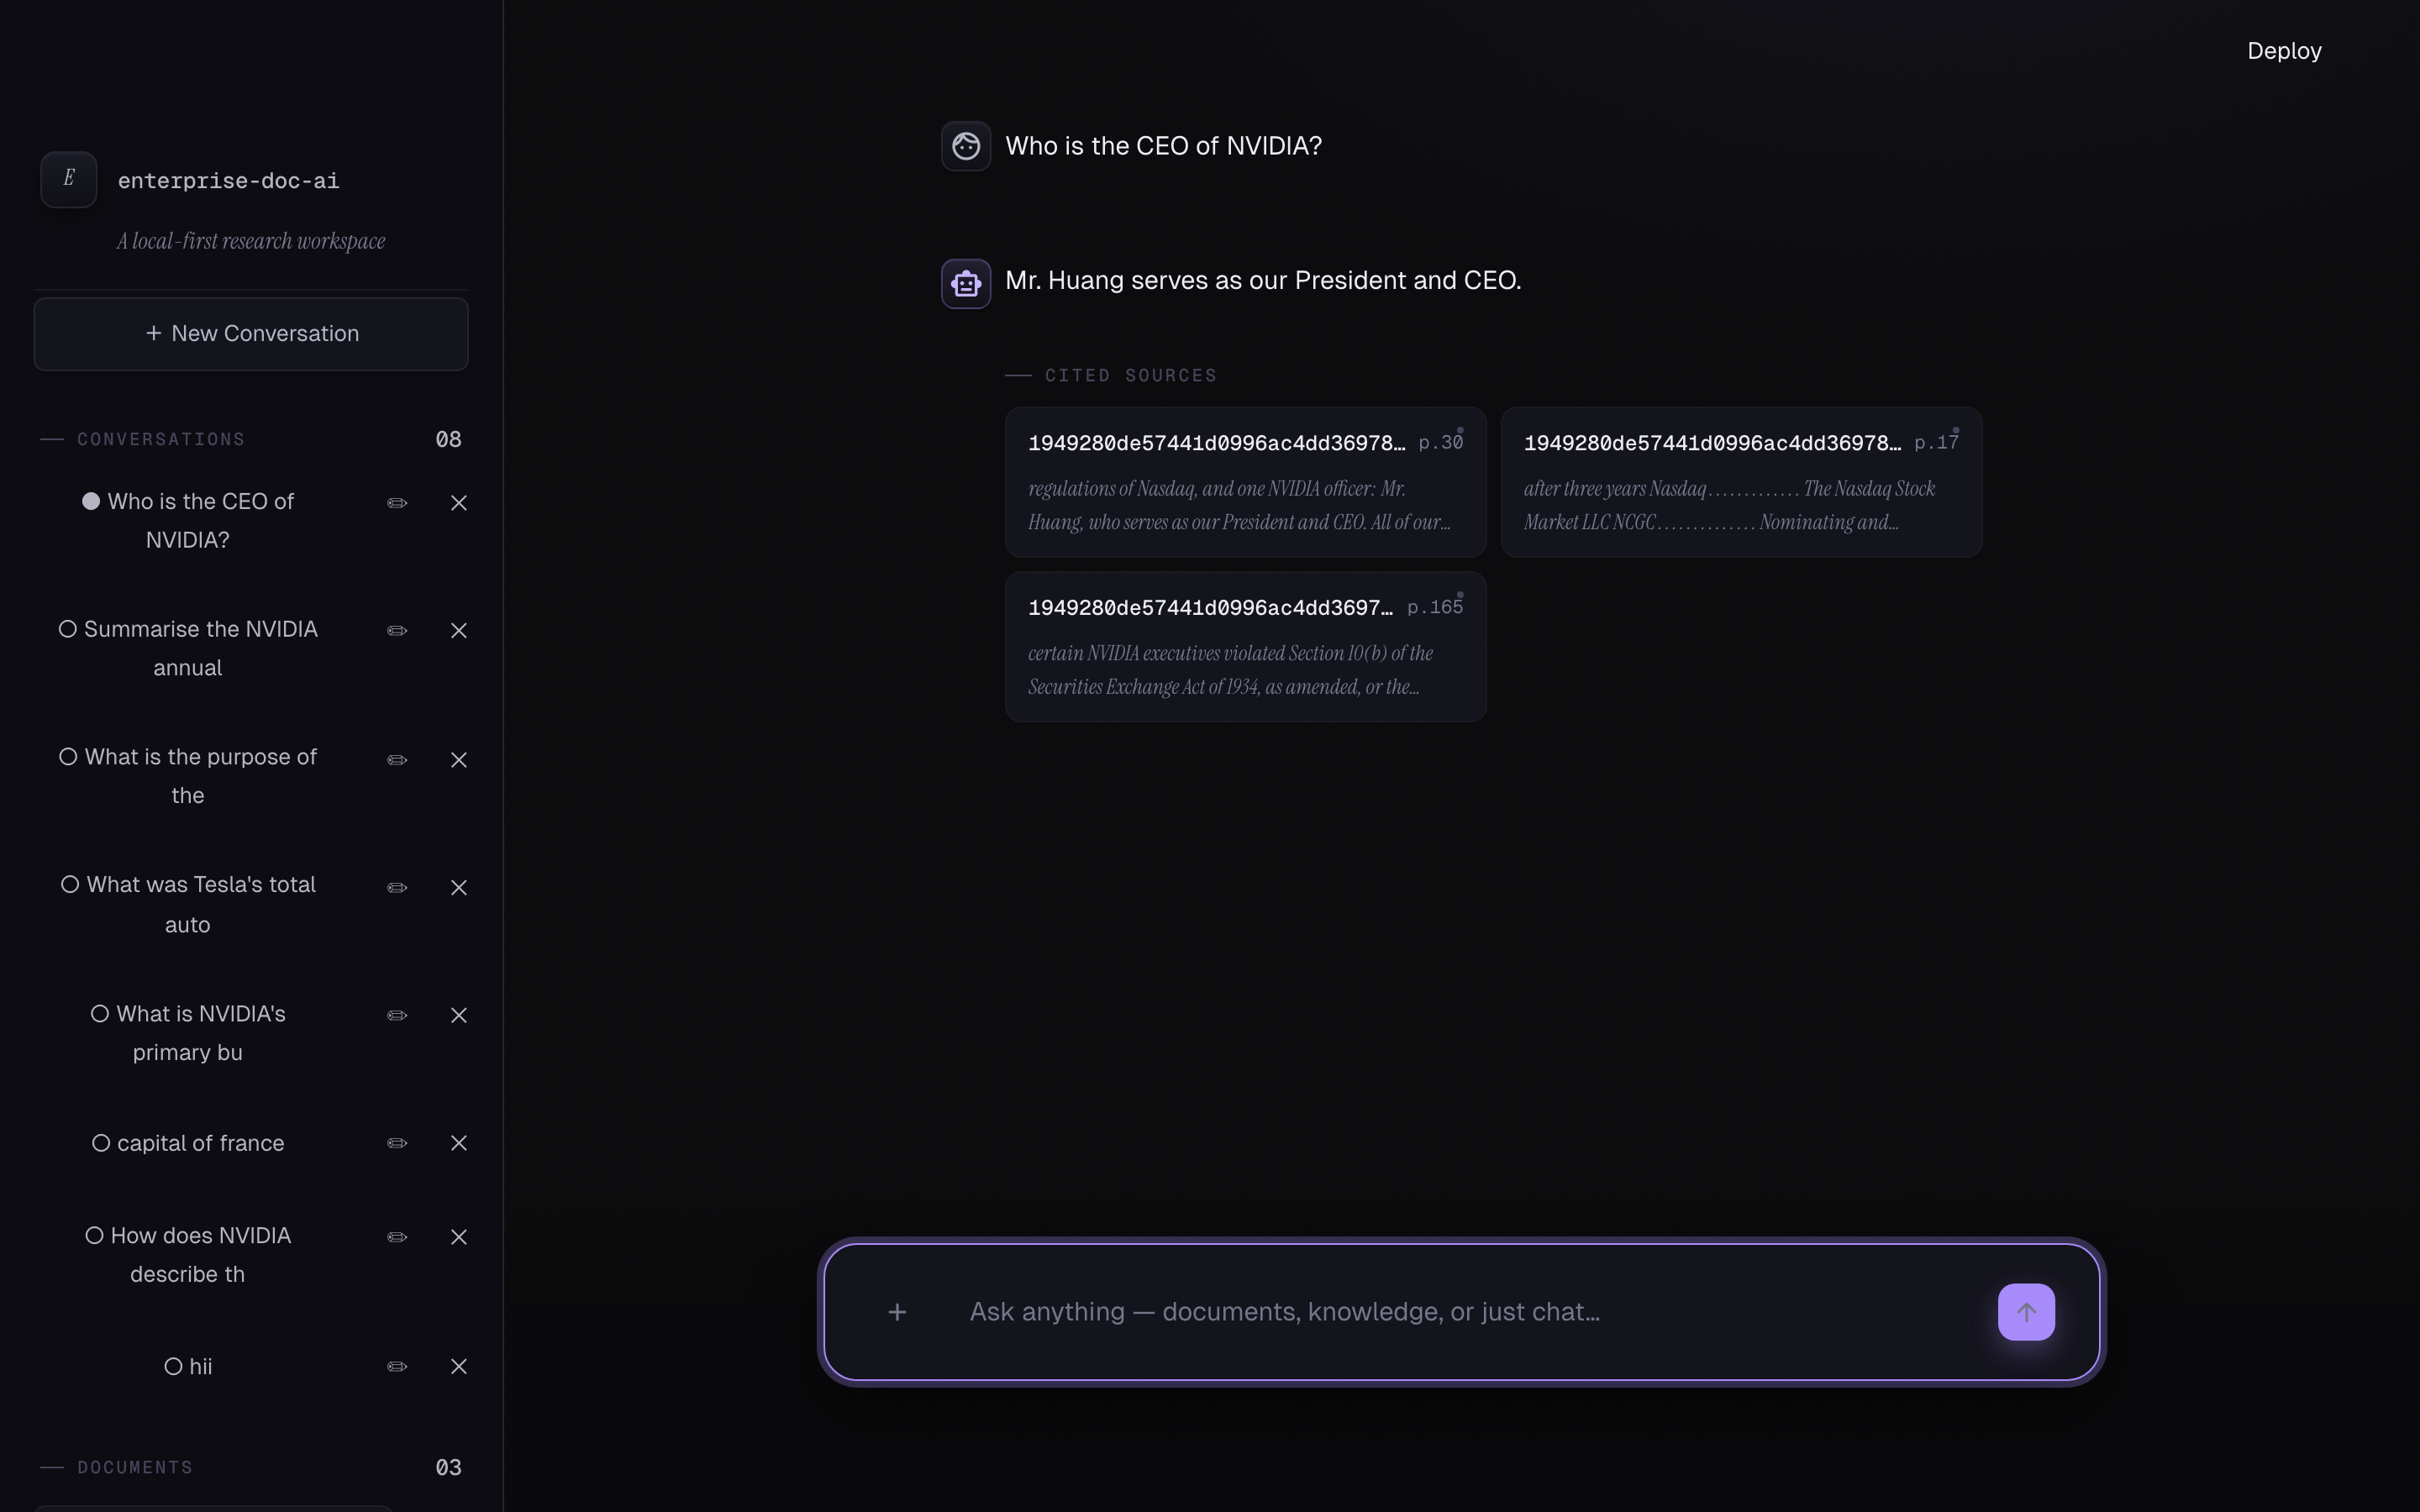
\includegraphics[width=\linewidth,height=4.6cm,keepaspectratio]{figures/02_nvidia_query.png}
\caption{\textsc{factual}: ``Who is the CEO of NVIDIA?''
\textbf{Answer:} ``Mr.\ Huang serves as our President and CEO.''}
\label{fig:nvidia}
\end{subcaptionblock}\hfill
\begin{subcaptionblock}{0.32\textwidth}
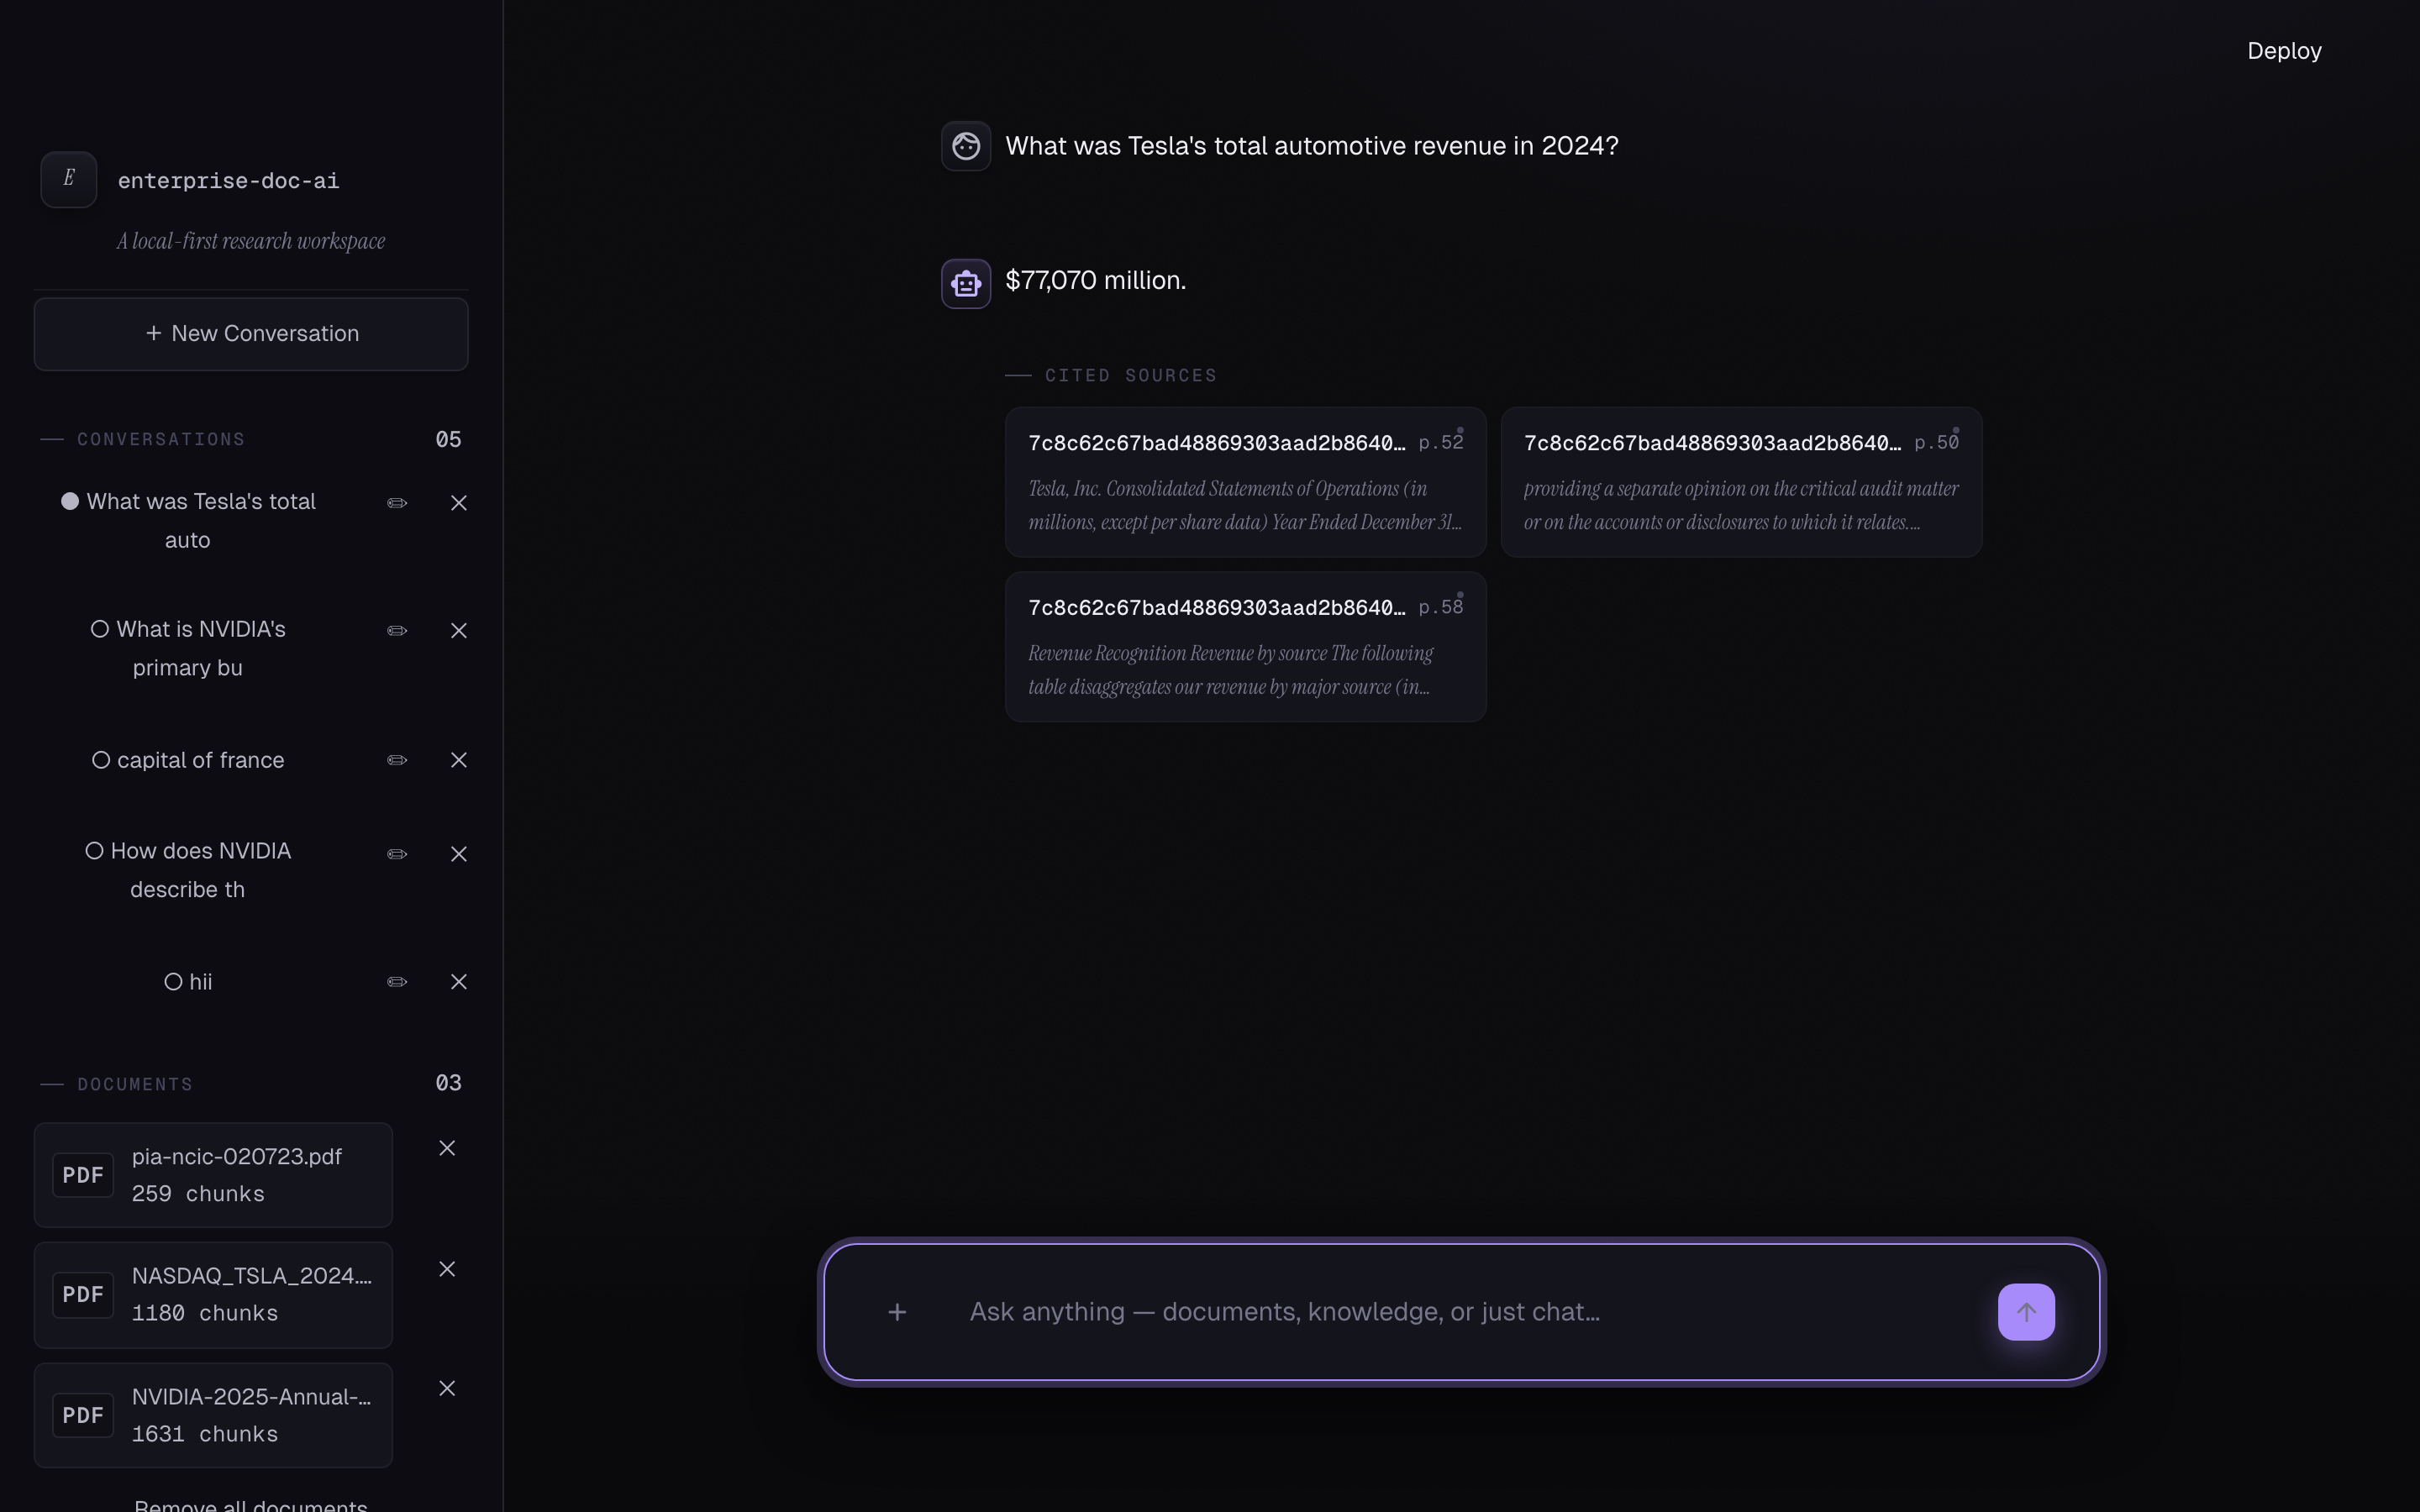
\includegraphics[width=\linewidth,height=4.6cm,keepaspectratio]{figures/03_tesla_query.png}
\caption{\textsc{numerical}: ``Tesla's total automotive revenue in 2024?''
\textbf{Answer:} ``\$77{,}070 million.''}
\label{fig:tesla}
\end{subcaptionblock}\hfill
\begin{subcaptionblock}{0.32\textwidth}
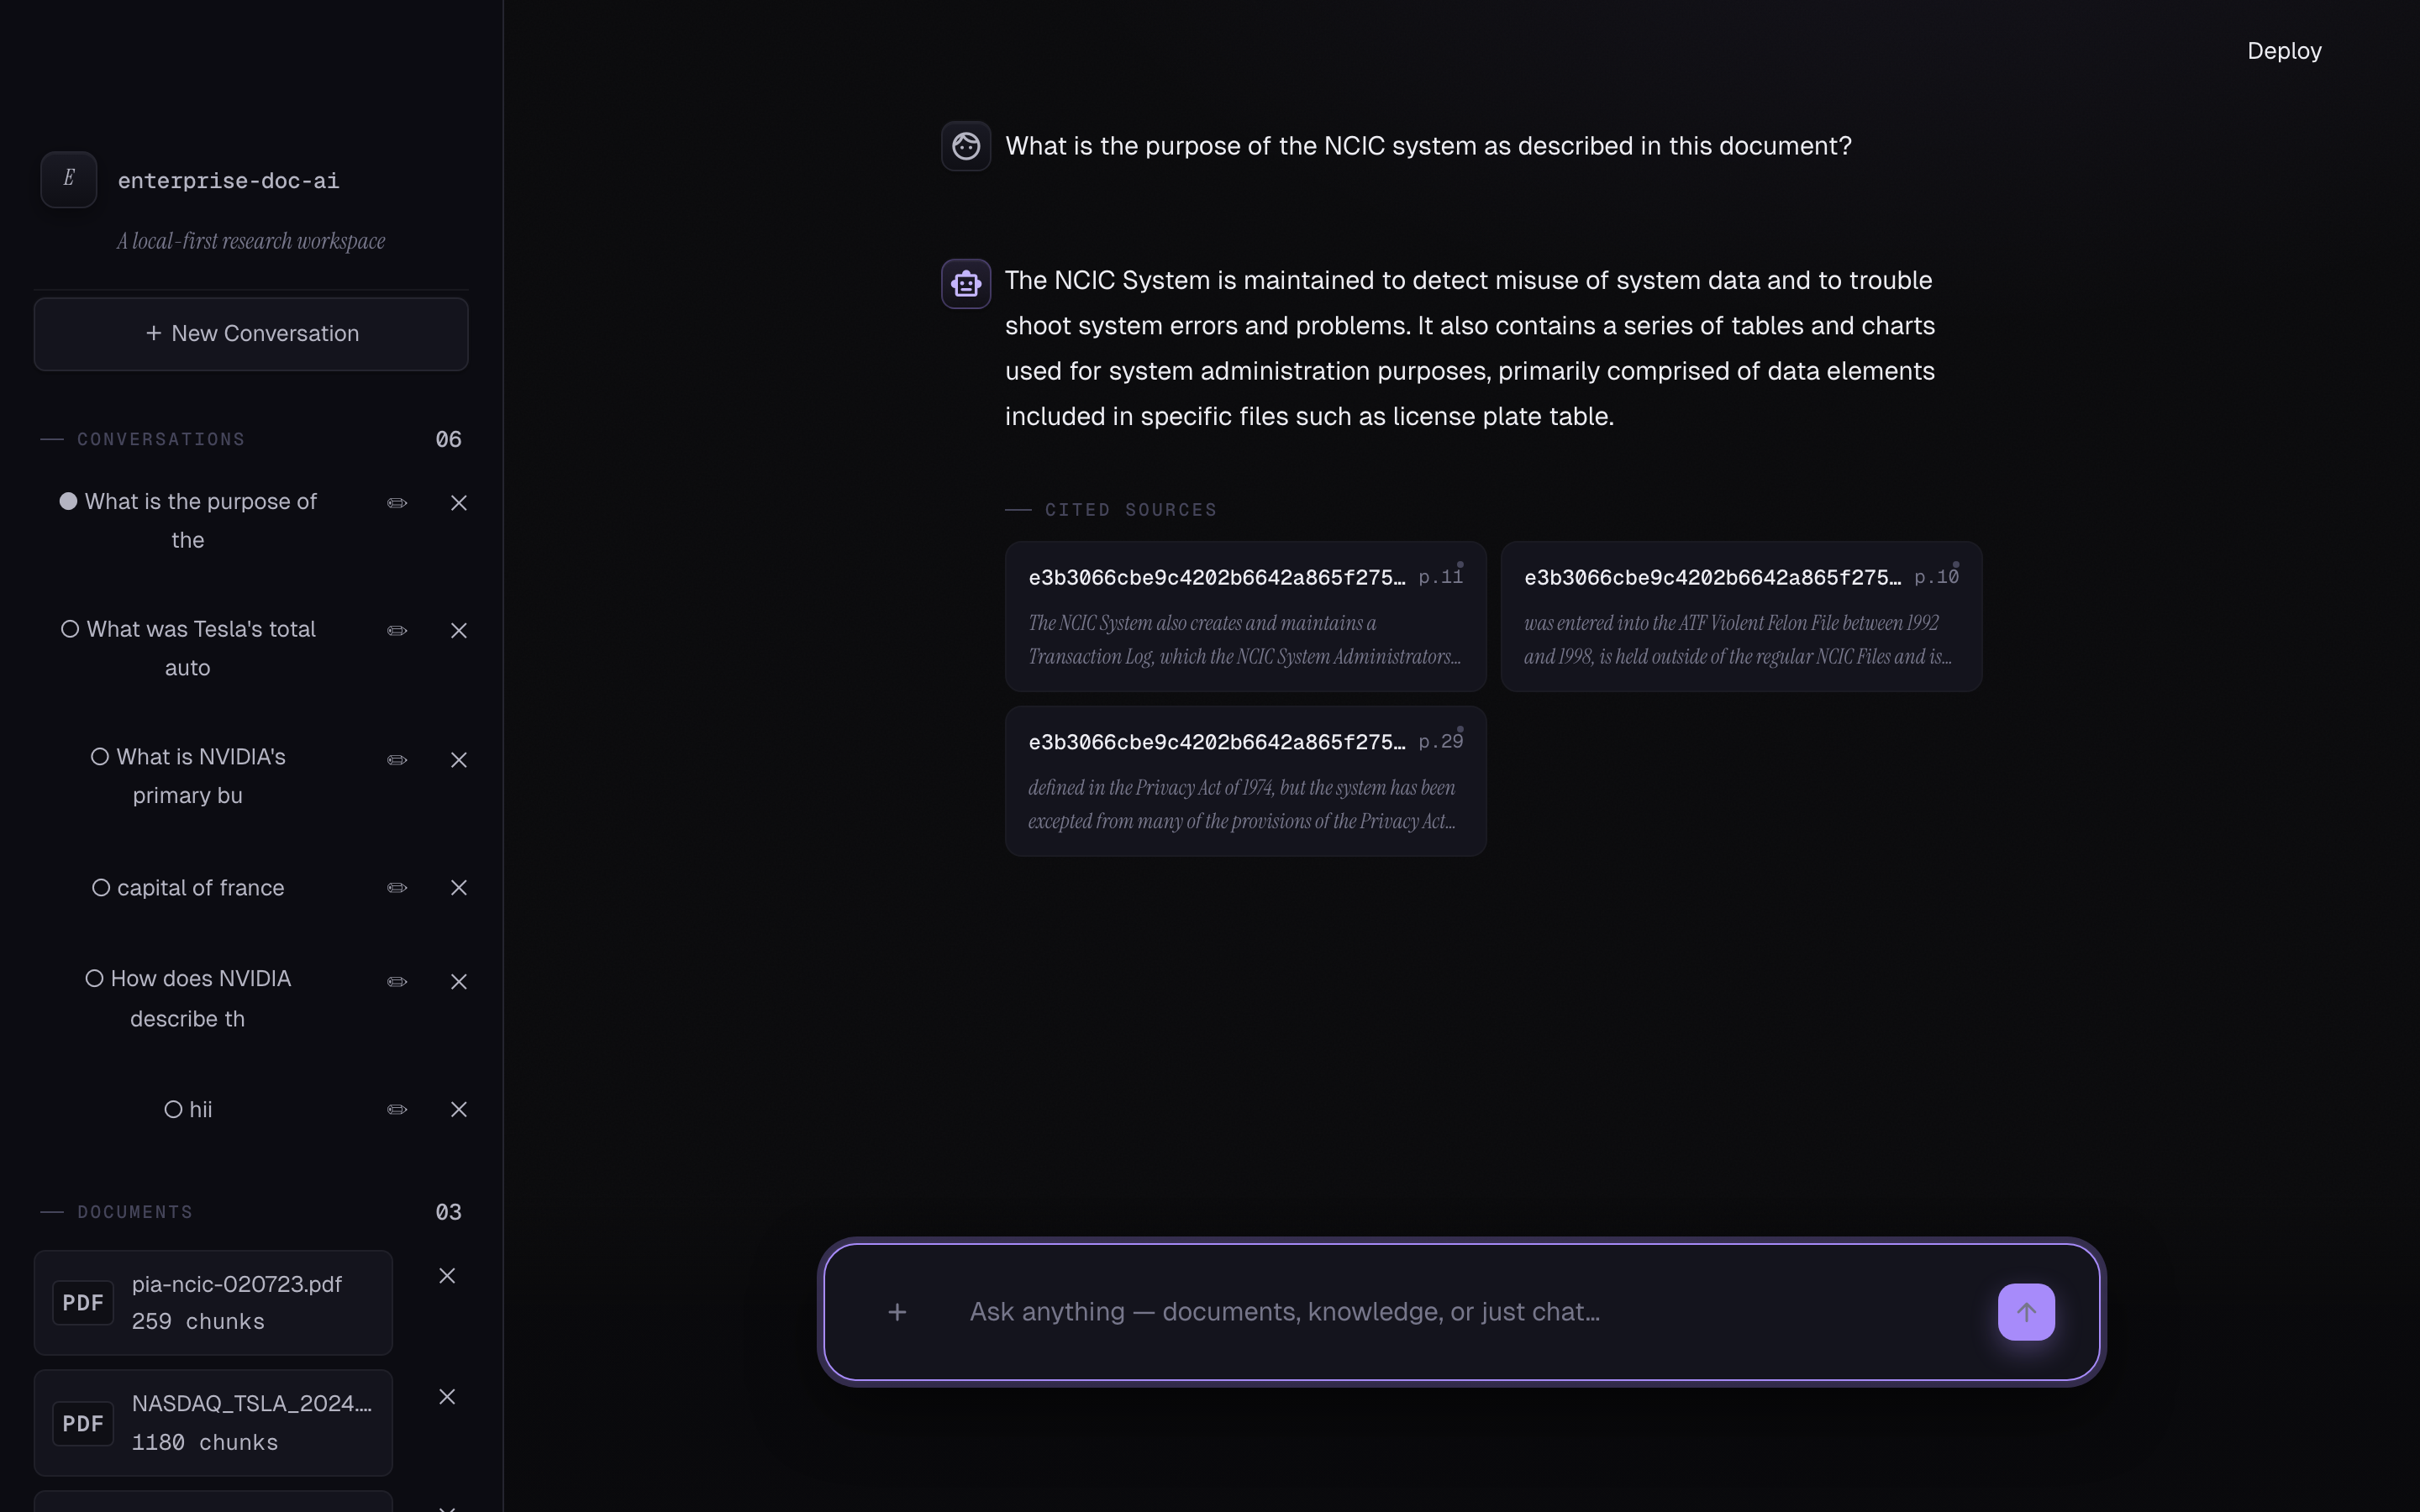
\includegraphics[width=\linewidth,height=4.6cm,keepaspectratio]{figures/04_ncic_query.png}
\caption{\textsc{reasoning}: ``Purpose of the NCIC system?''
\textbf{Answer:} ``Maintained to detect misuse of system data and to
troubleshoot system errors\,$\dots$''}
\label{fig:ncic}
\end{subcaptionblock}
\caption{Three grounded answers, one per PDF in the test corpus. Each
answer is accompanied by three source citations (file / page / snippet)
rendered from chunk metadata so the user can verify the fact at its source.}
\label{fig:demos}
\end{figure}

\paragraph{Hardware and latency.}
Apple~M2, 8\,GB RAM, no GPU. Indexing the NVIDIA report (1{,}631 chunks)
takes $\approx\!55$\,s; Tesla $\approx\!40$\,s; NCIC $\approx\!9$\,s. After
ingestion, factual queries take 5--8\,s, reasoning 8--12\,s, and summaries
12--18\,s. The first query after a cold start pays a one-time
$\approx\!3$\,s model-load tax inside Ollama.

\paragraph{Router and multi-turn.}
Figure~\ref{fig:multiturn} shows one conversation containing a document
summary (turn~1) and a chat greeting (turn~2). Turn~1 is sent to document
QA and produces a three-point grounded summary of the NVIDIA report;
turn~2 matches the greeting prefix and is sent to general chat with no
retrieval -- the model replies ``Hello! I'm here to help. How can I assist
you today?''.

\begin{figure}[h]
\centering
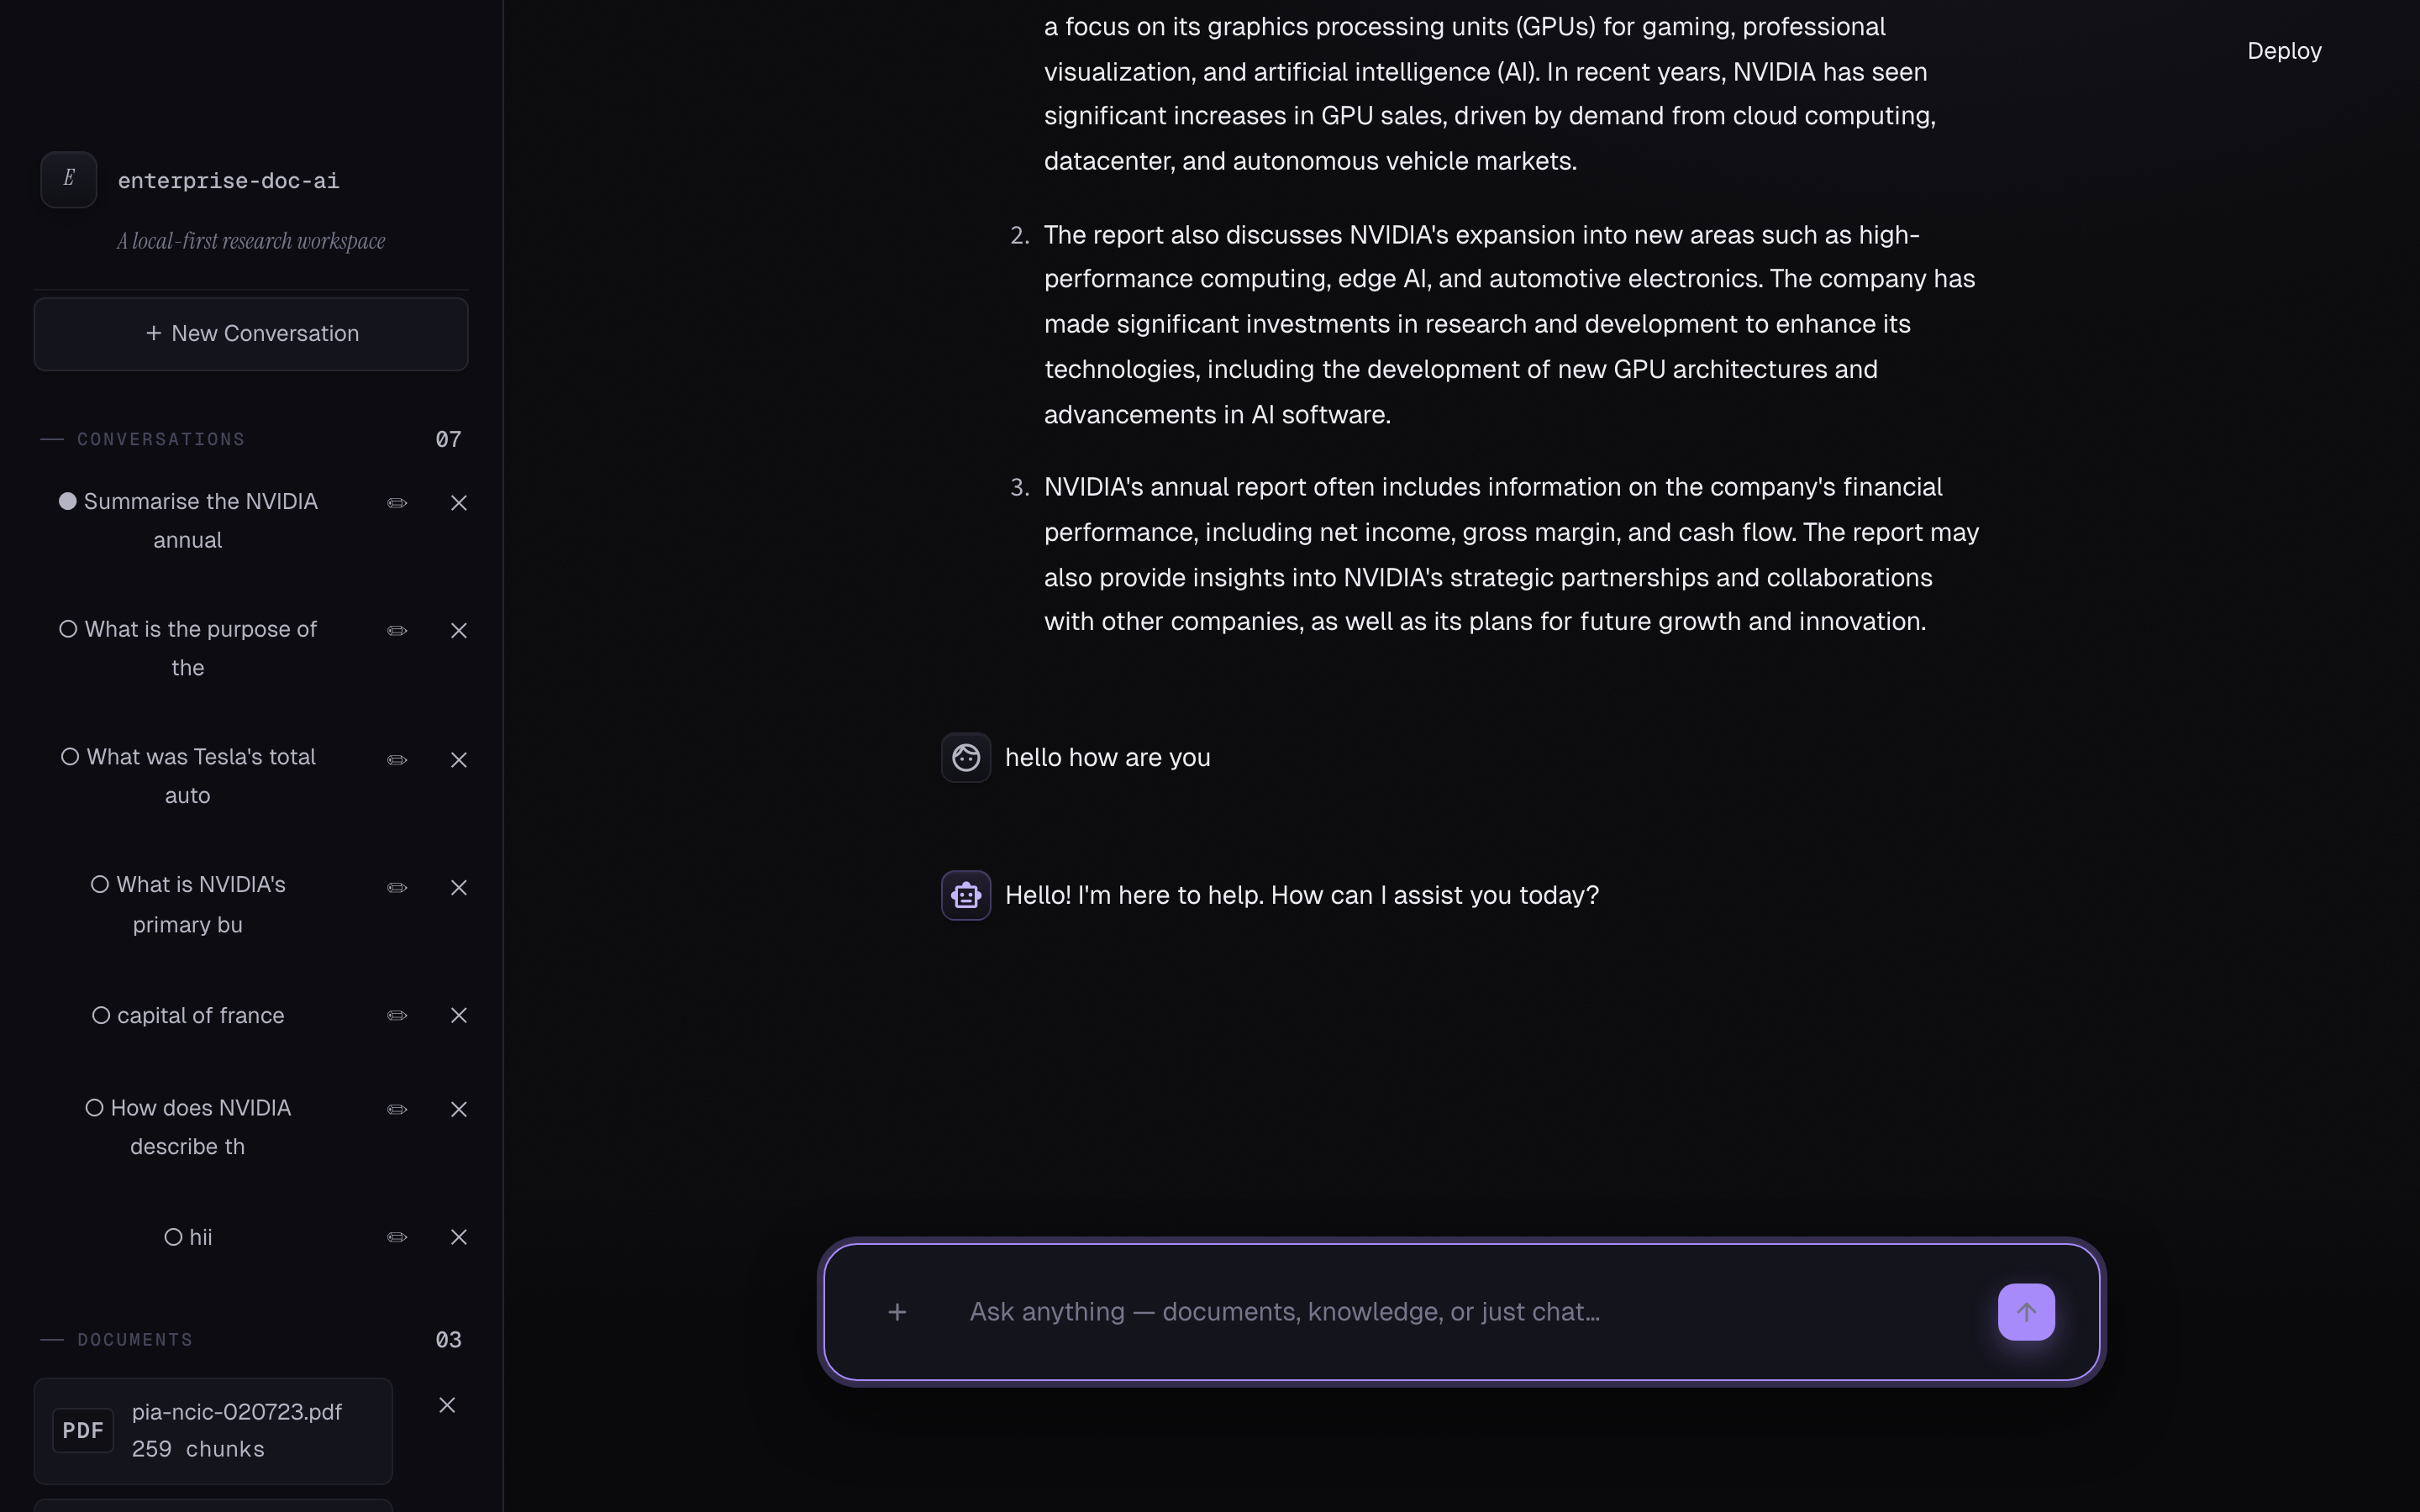
\includegraphics[width=0.75\linewidth,height=5.6cm,keepaspectratio]{figures/05_multi_turn_router.png}
\caption{One conversation crossing two routing branches. Turn~1 is grounded
against the NVIDIA Annual Report; turn~2 is a chat greeting that bypasses
retrieval entirely. The full conversation lives in SQLite, so both turns
appear in the same thread.}
\label{fig:multiturn}
\end{figure}

% =============================================================================
\section{Limitations, Future Work, and Conclusion}
\label{sec:disc}

\paragraph{Limitations.}
\texttt{llama3.2:3b} at four-bit quantisation is the smallest model we
found that produces fluent English; on harder queries it occasionally
paraphrases a fact instead of copying it. The router is rule-based and can
misclassify edge cases. The cross-encoder we use (\texttt{ms-marco-MiniLM-L-6-v2})
is small.

\paragraph{Future work.}
A stronger cross-encoder (\texttt{bge-reranker-base}) would lift retrieval
quality. Streaming responses via FastAPI server-sent events would change
the user's perceived latency from a 5--15\,s wait to an immediate first
token. A learned router would handle the edge cases the keyword router
misses. Multilingual support comes for free by swapping the embedding
model for \texttt{bge-m3}.

\paragraph{Conclusion -- the whole project, in six short paragraphs.}

\textbf{1.\;The problem.}\;
Private documents need a smart assistant, but hosted services upload the
file to a third-party server, charge per token of input and output, and
even when they use retrieval the small model still invents facts that
sound right. None of those failure modes is acceptable for a student or
researcher who wants to ask careful questions of confidential material.

\textbf{2.\;What we built.}\;
A FastAPI backend + Streamlit chat front-end in which \emph{every}
component --- the file parser, the BM25 keyword index, the dense
embeddings, the vector store, the LLM, and the conversation memory ---
runs on a single laptop. Once the model files are pulled, no network
connection is needed at query time.

\textbf{3.\;How we tested it.}\;
On three deliberately diverse PDFs that stress different parts of the
pipeline: the NVIDIA 2025 Annual Report (1{,}631 chunks of dense tech
prose, tests retrieval scale and hallucination guards), the Tesla 10-K
FY24 (1{,}180 chunks, financial-table heavy, tests the table-aware
chunker), and the FBI NCIC Privacy Impact Assessment (259 chunks,
government reasoning, tests open-ended ``what is the purpose of $X$''
questions) --- 3{,}070 chunks indexed together. The system works on any
user-supplied PDF, DOCX, TXT or image; these three are demonstration
cases.

\textbf{4.\;What broke and how we fixed it.}\;
Retrieval missed obvious chunks (fixed with hybrid BM25 + vector +
small domain bonuses); the small LLM invented hedge phrases such as
``could lead to'' (fixed with a 10-rule grounded prompt + regex opener
cleaner); verbatim quotes were paraphrased (fixed by bypassing the LLM
for the \textsc{extractive} and \textsc{provenance} query types);
financial tables collapsed into one unreadable line (fixed with a
6-line numeric-line heuristic in the chunker); and Milvus dropped its
connection after Mac sleep/wake (fixed by catching the specific error,
resetting and retrying, plus auto-rebuilding the vector store from
SQLite on startup).

\textbf{5.\;What works now.}\;
``Who is the CEO of NVIDIA?'' returns
\textit{``Mr.\ Huang serves as our President and CEO''} in 5--8\,s;
``Tesla's total automotive revenue in 2024?'' returns
\textit{``\$77{,}070 million''}; ``Purpose of the NCIC system?'' returns
a multi-sentence reasoning answer. Every answer carries three verifiable
source citations rendered next to it, so the user can always check the
fact at its origin.

\textbf{6.\;Why it matters.}\;
A complete retrieval-augmented generation pipeline --- parsing,
chunking, hybrid retrieval, query classification, grounded generation,
and conversation memory --- can run on a single 8\,GB laptop, on the
user's data, without sending a single byte to the cloud. That is the
local-first counterpart to hosted RAG services and the central
contribution of this project.

\end{document}
